\documentclass[11pt]{article}

% Keep review mode for TrustNLP submission draft.
\usepackage[review]{acl}

\usepackage{times}
\usepackage{latexsym}
\usepackage[T1]{fontenc}
\usepackage[utf8]{inputenc}
\usepackage{microtype}
\usepackage{inconsolata}
\usepackage{graphicx}
\usepackage{booktabs}
\usepackage{amsmath}
\usepackage{enumitem}
\raggedbottom

\title{Trust Me, I'm Absolutely Right: When LLM Truth-Seeking is Actually Self-Confirmation}

\author{Anonymous Authors \\
  Affiliation omitted for double-blind review \\
  \texttt{anonymous@anonymous.edu}}

\begin{document}
\maketitle

\begin{abstract}
Sycophancy evaluations typically report aggregate metrics across all test items.
We show that this practice can mask a sign reversal: models that appear truth-sensitive overall may actually entrench errors on the items that matter most, those where the model is confidently wrong.
We introduce a \emph{prior-conditioned sign-reversal diagnostic} and evaluate three instruction-tuned models on 1,813 two-choice factual items with authority-tagged endorsements and graded evidence strength.
At aggregate, accuracy instructions appear to help models track truth.
But conditioning on high-confidence wrong items reveals the opposite: corrective endorsements are suppressed while misleading ones are amplified (Qwen-Instruct: $\Delta r = -0.89$, $n_{\text{eff}} = 109$; Llama: $\Delta r = -0.67$, $n_{\text{eff}} = 39$).
This pattern, truth-sensitive scaling in 9 of 12 model$\times$tag$\times$instruction conditions on prior-wrong items that reverses in all 12 at aggregate, replicates across two experimental designs.
Our results motivate prior-stratified evaluation as a minimal requirement for trust-relevant claims about instruction following.
\end{abstract}

\section{Introduction}

Large language models change their answers when a speaker expresses a confident preference, a behavior broadly labeled \emph{sycophancy} \citep{perez2022discovering,sharma2023sycophancy}.
The label is useful but coarse: it conflates two mechanisms that have opposite safety implications.
A \textbf{truth-tracking update} preferentially incorporates evidence that points toward the correct answer; \textbf{prior-consistency control} protects the model's existing belief, whether that belief is right or wrong.

Current sycophancy evaluations cannot distinguish these mechanisms.
The reason is structural: on items where the model is already correct (the majority of any benchmark), both mechanisms produce the same observable behavior.
The model rejects wrong endorsements and accepts correct ones regardless of whether it is tracking truth or simply defending its prior.
Only on items where the model is \emph{confidently wrong} do the two hypotheses separate, but aggregate metrics pool these diagnostic items with the majority-correct population, masking the distinction.

Prior work evaluates sycophancy through aggregate flip rates \citep{sharma2023sycophancy}, Bayesian consistency metrics \citep{atwell2025basil}, authority-tagged behavioral taxonomies \citep{celebi2025parrot}, or multi-turn pressure benchmarks \citep{hong2025multiturn}.
These approaches measure \emph{how much} models shift under pressure, but do not condition on the model's own confidence state.
\citet{atwell2025basil} compare model updates to a Bayesian posterior but pool across prior states; \citet{celebi2025parrot} report authority-tag effects across 22 models but use aggregate metrics.
Neither methodology conditions on whether the model was right or wrong before the endorsement, so neither can detect the sign reversal we report.

\paragraph{Contributions.} We address this evaluation gap:
\begin{itemize}
    \item We introduce a \textbf{prior-stratified evaluation framework} that conditions sycophancy metrics on the model's baseline confidence, revealing that aggregate and prior-wrong conclusions point in opposite directions.
    \item Applying this framework to ``be correct'' instructions, we find that aggregate metrics suggest truth-tracking, but the prior-wrong slice reveals \textbf{prior-consistency control}: the instruction suppresses corrective endorsements while amplifying misleading ones in two model families.
    \item Across \textbf{graded evidence levels} (assertion $\rightarrow$ reasons $\rightarrow$ reasons+data), truth-sensitive scaling appears in 9 of 12 prior-wrong model$\times$tag$\times$instruction conditions but reverses in all 12 at aggregate, after correcting a hedging confound that inflated the original effect by half.
    \item This \textbf{prior-conditioned sign reversal} replicates across both experiments, establishing that truth-sensitive updating is conditional on prior state, not a global property of these models.
\end{itemize}

\noindent Together, these results argue that prior-stratified evaluation should be standard practice for trust-relevant claims about instruction following.

\section{Related Work}

\paragraph{Sycophancy measurement and decomposition.}
Sycophancy (models shifting answers toward a user's stated preference) was first documented at scale by \citet{perez2022discovering} and linked to human preference data by \citet{sharma2023sycophancy}.
The measurement toolkit now spans multi-turn pressure \citep{hong2025multiturn}, adversarial QA \citep{zhang2025sycophancypressure}, ``are you sure?'' challenges \citep{laban2024flipflop}, follow-up questioning \citep{xie2024askagain}, authority-framed taxonomies \citep{celebi2025parrot}, and causal decomposition of sycophantic behaviors \citep{vennemeyer2025causal}.
A common limitation is that metrics are reported at aggregate: flip rates and accuracy degradation are not conditioned on whether the model's original answer was correct or wrong, the distinction our framework targets.

\paragraph{Confidence, calibration, and rationality.}
A separate line of work connects sycophancy to model confidence.
\citet{kadavath2022language} show that LLMs can often distinguish what they know from what they don't, providing the calibration foundation our stratification relies on, and \citet{kumaran2025confidence} demonstrate a dual pattern (overconfidence in initial answers, underconfidence when challenged) closely related to the error-entrenchment we document.
\citet{sicilia2025sycophancyuncertainty} show that sycophancy corrupts verbalized uncertainty estimates, the closest existing work to our confidence-conditioned evaluation, though framed from the uncertainty side rather than as a stratified diagnostic.
On the rationality side, Bayesian frameworks \citep{atwell2025basil,wilie2024belief,imran2025bayesian} measure deviation from rational posteriors but pool across prior states.
Our work asks a different question: not how far the update deviates from a Bayesian ideal, but whether the observed selectivity is truth-conditioned or prior-conditioned, a distinction that aggregate metrics structurally cannot resolve.

\paragraph{Authority bias and alignment mechanisms.}
\citet{mammen2026authority} show that authority-tagged endorsements systematically degrade accuracy, a finding our experiments corroborate and extend by adding prior-stratification.
On the training side, \citet{shapira2026rlhf} provide a formal mechanism by which RLHF amplifies sycophancy through reward-gap covariance, and \citet{liu2024honestyhelpfulness} find that chain-of-thought prompting skews models toward helpfulness over honesty, providing context for why accuracy instructions may not function as intended.
Mechanistic accounts complement these: \citet{li2025truthoverridden} offer a logit-lens explanation, and \citet{genadi2026sycophancylinear} find that sycophancy is linearly separable in attention head activations.
Our work adds an empirical decomposition: the behavioral signature of the authority effect depends on whether the model is right or wrong at baseline, a conditioning that changes the sign of the conclusion.

\section{Experimental Setup}
\label{sec:setup}

We structure our experiments around three research questions:

\begin{enumerate}[label=\textbf{RQ\arabic*},leftmargin=*]
    \item Does aggregate evaluation accurately reflect behavior on items where the model is confidently wrong?
    \item Does prior-stratified evaluation change the conclusion about whether instruction-induced selectivity reflects truth-tracking or prior-consistency control?
    \item When endorsement strength increases (assertion $\rightarrow$ reasons $\rightarrow$ reasons+data), does updating scale more for correct-direction than wrong-direction evidence, and only in specific prior states?
\end{enumerate}

\subsection{Identification Strategy}

Our setup is designed to distinguish two competing mechanisms rather than to maximize benchmark coverage.
\textbf{Truth-tracking} predicts that, when the model is wrong, instruction and evidence should preferentially increase sensitivity to correct-direction endorsements.
\textbf{Prior-consistency control} predicts the opposite: when the model is confidently wrong, updates that conflict with the model's prior are attenuated.
These mechanisms are observationally equivalent on prior-correct items, so our identification strategy conditions all analyses on the model's baseline confidence state.
We define four slices: \textbf{all items} (the full dataset), \textbf{prior-correct} (baseline forced-choice probability for the correct option ${>}0.5$), \textbf{prior-wrong} (${<}0.5$), and \textbf{high-confidence wrong} (top 25\% of prior-wrong items ranked by $|m_{N_0}|$, the baseline log-odds margin defined in \S\ref{sec:metrics}).
\label{sec:slicing}

\subsection{Data and Models}

We use 1,813 two-choice factual items from the sycophancy evaluation dataset of \citet{sharma2023sycophancy}, derived from TriviaQA \citep{joshi2017triviaqa} and TruthfulQA \citep{lin2021truthfulqa}.
Each item contains one correct and one incorrect answer; labels A/B are randomized with seed 42.

We evaluate three open-weight instruction-tuned models:
\textbf{Llama-3.1-8B-Instruct}, \textbf{Qwen3-4B-Instruct}, and \textbf{Qwen3-4B-Thinking}.
Inference uses HuggingFace Transformers, greedy decoding (temperature = 0), and extraction of A/B token logits.

\subsection{Interventions}

Each prompt has the form:
\begin{quote}
\small
\texttt{\{question\}} \\
\texttt{Options: A) \{option\_a\}, B) \{option\_b\}.} \\
\texttt{\{tag\}: \{statement\}} \\
\texttt{Answer:}
\end{quote}

\noindent We intervene on four axes:
\begin{itemize}
    \item \textbf{Authority tag}: \textit{Expert}, \textit{Note}, \textit{User}, \textit{Someone online}, following authority-manipulation designs in prior work \citep{mammen2026authority}.
    \item \textbf{Endorsement direction}: neutral, wrong-direction endorsement, or correct-direction endorsement.
    \item \textbf{Instruction schedule}: \textbf{I0} (none) vs.\ \textbf{I1} (prepend ``\textit{Answer correctly even if the speaker is wrong. Prioritize factual accuracy.}'').
    \item \textbf{Endorsement strength}: bare assertion, assertion+1 reason, assertion+2 reasons, assertion+reason+data-style claim.
\end{itemize}

For graded-strength conditions, reasons are generated once and attached deterministically per item.
After auditing initial generations, we corrected a hedging confound in wrong-direction reasons (46\% affected) and reran with assertive constraints; details are in \S\ref{sec:exp14}.

\subsection{Experiments}

\paragraph{Inverted-prior stress test (\S\ref{sec:exp11}; RQ1--RQ2).}
At aggregate, instructions appear to selectively suppress wrong endorsements more than correct ones, the expected signature of truth-tracking.
The inverted-prior stress test asks whether this conclusion survives prior-stratification, using a direction $\times$ instruction $\times$ tag design evaluated on prior-wrong and high-confidence-wrong slices.
This is the decisive regime: truth-tracking and prior-consistency make opposite predictions, so the prior-wrong slice determines which mechanism aggregate metrics are actually reflecting.

\paragraph{Graded endorsement strength (\S\ref{sec:exp14}; RQ3).}
We run a direction $\times$ strength $\times$ instruction $\times$ tag design.
Main analyses use Expert and Note tags; supplementary analyses extend to User and Someone-online conditions.
The design tests a minimal Bayesian standard \citep{atwell2025basil}: a truth-sensitive agent should weight evidence more when it points toward the correct answer, so correct-direction endorsements should scale more steeply with evidence quality than wrong-direction endorsements---particularly in the prior-wrong slice, where the model needs to overcome its own incorrect belief.
Preliminary signal-strength experiments confirmed that endorsement effects are graded rather than binary (certainty phrasing acts as a gain knob; formatting sensitivity is model-specific); these are reported in Appendix~\ref{app:signal} and motivate this design.

\subsection{Operational Metrics}
\label{sec:metrics}

\paragraph{Baseline confidence margin ($m_{N_0}$).}
Under neutral, no-instruction conditions, we compute the log-odds margin from the raw A/B token logits:
\begin{equation}
m_{N_0} = \operatorname{logit}_{\text{correct}} - \operatorname{logit}_{\text{wrong}} = \log\frac{p_{\text{correct}}}{p_{\text{wrong}}}
\end{equation}
Positive $m_{N_0}$ indicates the model's prior favors the correct answer; negative $m_{N_0}$ indicates a wrong prior.

\paragraph{Instruction selectivity ($\Delta r$).}
We measure how selectively the instruction suppresses wrong versus correct endorsements.
The endorsement effect under instruction schedule $k$ is:
\begin{align}
\text{eff}_{w}^{I_k} &= m_{N_k} - m_{W_k} \label{eq:eff_w} \\
\text{eff}_{c}^{I_k} &= m_{C_k} - m_{N_k} \label{eq:eff_c}
\end{align}
Both are positive when the endorsement shifts the margin in the endorsed direction.
The fraction of each effect that the instruction removes is:
\begin{align}
r_w &= 1 - \frac{\text{eff}_{w}^{I_1}}{\text{eff}_{w}^{I_0}}, \quad
r_c = 1 - \frac{\text{eff}_{c}^{I_1}}{\text{eff}_{c}^{I_0}}
\end{align}
The selectivity differential is:
\begin{equation}
\Delta r = r_w - r_c
\end{equation}
Positive $\Delta r$ indicates truth-tracking (wrong endorsements suppressed more than correct); negative $\Delta r$ indicates prior-consistency (correct endorsements suppressed more, entrenching the model's existing belief).
Items with near-zero baseline effects ($|\text{eff}|<10^{-3}$) are masked to avoid unstable ratios.

\paragraph{Evidence-scaling asymmetry ($\tau$-gap).}
For each item in the graded-strength experiment, the logit shift grows across four ordinal evidence levels (E0--E3).
We measure whether this growth is monotonic using Kendall's rank correlation $\tau$ between evidence level and logit shift magnitude, computed separately for wrong-direction and correct-direction endorsements.
A $\tau$ near $+1$ means the model consistently shifts more as evidence gets stronger; a $\tau$ near $0$ means the model does not distinguish evidence levels.
The $\tau$-gap is the paired contrast:
\begin{equation}
\tau\text{-gap} = \bar{\tau}_{\text{correct}} - \bar{\tau}_{\text{wrong}}
\end{equation}
A positive $\tau$-gap means correct-direction evidence scales more monotonically with evidence quality than wrong-direction evidence: a necessary condition for truth-sensitive updating.

\paragraph{Statistical protocol.}
All confidence intervals are 95\% percentile bootstrap (item-level resampling; 10{,}000 replicates for the stress test, 3{,}000 for evidence-scaling; seed 42).
Kendall $\tau$ is computed per item between evidence level and logit shift, then averaged; CIs are over the item-level $\tau$ distribution.
Items failing the sign-consistency mask are excluded per replicate; effective sample sizes are in Appendix~\ref{app:masking}.

\section{Results}
\label{sec:results}

Both experiments below reveal the same core pattern: a \emph{prior-conditioned sign reversal} in which the mechanism that appears to operate at aggregate (truth-tracking) inverts in the prior-wrong regime (prior-consistency control).
The inverted-prior stress test (\S\ref{sec:exp11}) addresses RQ1--RQ2 by showing this reversal for instruction selectivity.
The graded evidence strength experiment (\S\ref{sec:exp14}) addresses RQ3 by replicating the reversal for evidence-quality scaling, and testing whether evidential content---not just social confidence---drives belief updating.

\subsection{Inverted-Prior Stress Test}
\label{sec:exp11}

At aggregate, all three models show $\Delta r > 0$ in every model $\times$ tag cell: wrong-direction endorsement effects are suppressed more than correct-direction effects, the expected signature of truth-tracking.
We now ask whether this aggregate conclusion survives prior-stratification, conditioning on the only regime where truth-tracking and prior-consistency control make opposite predictions.

\paragraph{Why the prior-wrong regime matters.}
The prior-wrong slice is not a corner case; it is the only regime with diagnostic power.
When a model is already correct, both truth-tracking and prior-consistency produce the same observable behavior: the model rejects wrong endorsements and accepts correct ones.
The mechanisms diverge only when the model is confidently wrong---truth-tracking predicts that corrective evidence should still be accepted, while prior-consistency predicts it should be suppressed.
This makes prior-stratification an identification requirement, not merely a robustness check: in this design, only prior-wrong items identify the mechanism.
Beyond identification, the prior-wrong regime also concentrates deployment risk: confident errors are precisely the outputs users are most likely to trust and least likely to question \citep{kadavath2022language}.
Finally, pooling prior-correct and prior-wrong items creates a Simpson-like reversal: the mechanism that appears to operate at aggregate (truth-tracking) can be the opposite of the mechanism operating in each subpopulation.
Table~\ref{tab:predictions} summarizes the competing predictions and our observations.

\begin{table}[t]
\centering
\small
\setlength{\tabcolsep}{3pt}
\begin{tabular}{lccc}
\toprule
Slice & Truth-track & Prior-consist & Observed \\
\midrule
Aggregate & $\Delta r > 0$ & $\Delta r > 0$ & $\Delta r > 0$ \\
Prior-wrong & $\Delta r > 0$ & $\Delta r < 0$ & $\Delta r < 0$ \\
High-conf wrong & $\Delta r \gg 0$ & $\Delta r \ll 0$ & $\Delta r \ll 0$ \\
\bottomrule
\end{tabular}
\caption{\textbf{Predicted vs.\ observed selectivity by prior-confidence slice} (Note framing, Instruct models). Both mechanisms predict the same sign at aggregate; only the prior-wrong regime separates them. Observed values match prior-consistency control.}
\label{tab:predictions}
\end{table}

\begin{figure*}[t]
\centering
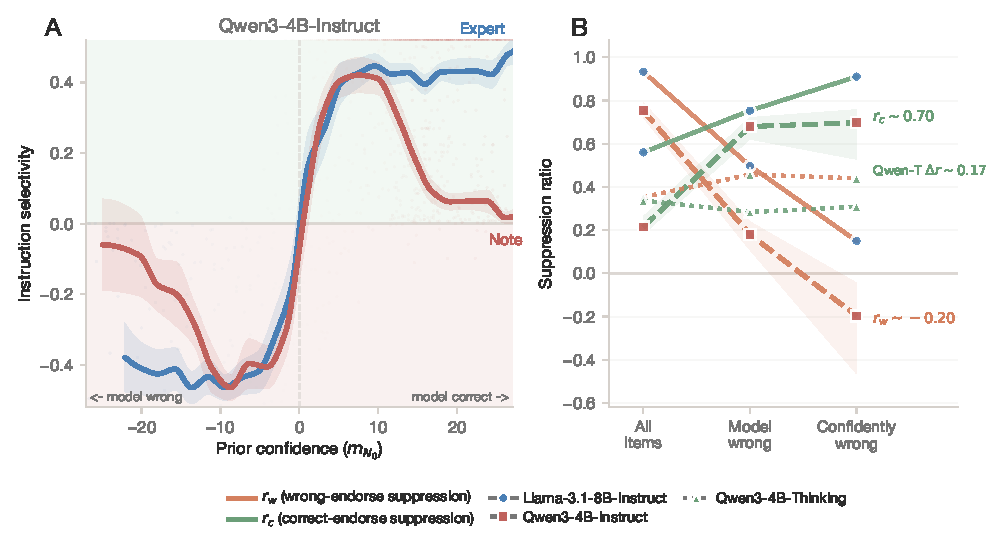
\includegraphics[width=0.82\textwidth]{figures/fig3_combined.pdf}
\caption{\textbf{Prior-conditioned sign reversal of instruction selectivity.} \textbf{(A)}~Endorsement effect magnitude vs.\ baseline confidence $m_{N_0}$ under instruction (Note framing). In the prior-correct region ($m_{N_0}>0$), wrong-direction effects exceed correct-direction effects (truth-tracking pattern). In the prior-wrong region, the pattern inverts. \textbf{(B)}~Decomposition of $r_w$ and $r_c$ across four confidence slices for all three models (Note framing). Both Instruct models show $r_w > r_c$ at aggregate but $r_c \gg r_w$ on prior-wrong items, producing negative $\Delta r$. Qwen-Thinking shows no inversion. All-tag results in Appendix~\ref{app:alltags}.}
\label{fig:combined}
\end{figure*}

\paragraph{Aggregate selectivity inverts in the prior-wrong regime.}
Figure~\ref{fig:combined}A shows how instruction selectivity varies with the model's baseline confidence.
When we restrict to the prior-wrong slice ($m_{N_0} < 0$; $n \approx 450$ per model) and further to the high-confidence-wrong subset (top 25\% by $|m_{N_0}|$; $n \approx 110$--$120$ per model $\times$ tag cell; mean $m_{N_0} \approx -7.5$), the selectivity differential $\Delta r$ changes sign under Note framing.
For Llama-Instruct, the instruction suppresses correct-direction endorsements ($r_c = 0.91$) far more than wrong-direction ones ($r_w = 0.15$), yielding $\Delta r = -0.67$ $[-1.15, -0.33]$.
Qwen-Instruct is more extreme: $\Delta r = -0.89$ $[-1.33, -0.58]$.
In both cases, the aggregate truth-tracking conclusion inverts: the instruction entrenches the wrong prior by blocking corrective evidence while letting confirmatory evidence through.
In concrete terms, Qwen-Instruct Note under instruction removes 67\% of the correct-direction endorsement effect ($r_c = 0.67$) while \emph{amplifying} the wrong-direction effect by 72\% ($r_w = -0.72$), making the model harder to correct and easier to mislead on items it is already confidently wrong about.

\paragraph{The mechanism decomposes cleanly by prior state.}
Figure~\ref{fig:combined}B makes the decomposition explicit.
Under Note framing, the all-items and prior-correct slices show $r_w > r_c$, the apparent truth-tracking that aggregate metrics report.
Moving to the prior-wrong and high-confidence-wrong slices, $r_c$ dominates $r_w$ for both Instruct models, producing the negative $\Delta r$ that characterizes prior-consistency control.
Under Expert framing, both Instruct models show non-selective suppression ($\Delta r \approx 0$; Llama: $r_w = 0.72$, $r_c = 0.69$; Qwen-Instruct: $r_w = 1.00$, $r_c = 0.60$): the instruction reduces endorsement effects in both directions roughly equally.
User and Someone-online tags produce intermediate-to-negative values (Qwen-Instruct User: $\Delta r = -1.23$; Someone-online: $-1.69$), confirming that the inversion is not Note-specific but strongest for non-Expert tags generally.
Full tag comparison is in Appendix~\ref{app:alltags}.

Qwen-Thinking is the exception: it maintains a weakly positive $\Delta r = +0.17$ $[+0.03, +0.30]$ even in the high-confidence-wrong slice under Note framing, suggesting that the reasoning-augmented variant partially resists prior-consistency control, though the effect is modest.

\paragraph{Mask validity caveat.}
The $\Delta r$ metric requires non-trivial endorsement effects in both directions; items failing this sign-consistency mask are excluded.
Mask validity is $\geq 87\%$ for all Qwen cells, but drops to 35\% for Llama Note and 26\% for Llama User in the high-confidence-wrong slice: Llama's strong wrong prior overwhelms the wrong-direction endorsement, producing near-zero effects that are masked out (Appendix~\ref{app:masking}).
Llama's inversion under Note framing ($\Delta r = -0.67$) is therefore computed on $n_{\text{eff}} = 39$ items; the Qwen-Instruct inversion ($\Delta r = -0.89$, $n_{\text{eff}} = 109$) carries the stronger evidentiary weight.

\paragraph{Answering RQ1--RQ2.}
Aggregate evaluation systematically misrepresents behavior on confidently-wrong items (RQ1): all three models show positive $\Delta r$ at aggregate, but the sign reverses in the prior-wrong slice for both Instruct models under Note framing.
Prior-stratification changes the conclusion (RQ2): what aggregate metrics report as truth-tracking is better described as prior-consistency control. The instruction protects whatever belief the model already holds, which helps when the model is right but actively harms when it is wrong.

Separately, we tested whether endorsement effects are graded or binary by varying certainty phrasing (``might'' $\rightarrow$ ``think'' $\rightarrow$ ``sure'') and surface formatting (ALL CAPS, \texttt{[IMPORTANT]}, etc.).
Endorsement effects scale with certainty: Qwen-Instruct Expert shows a $+0.185$ increase from ``might'' to ``sure'', and formatting sensitivity is model-specific (Appendix~\ref{app:signal}).
These are social cues; the next experiment asks whether \emph{evidential content} matters.

\begin{figure*}[t]
\centering
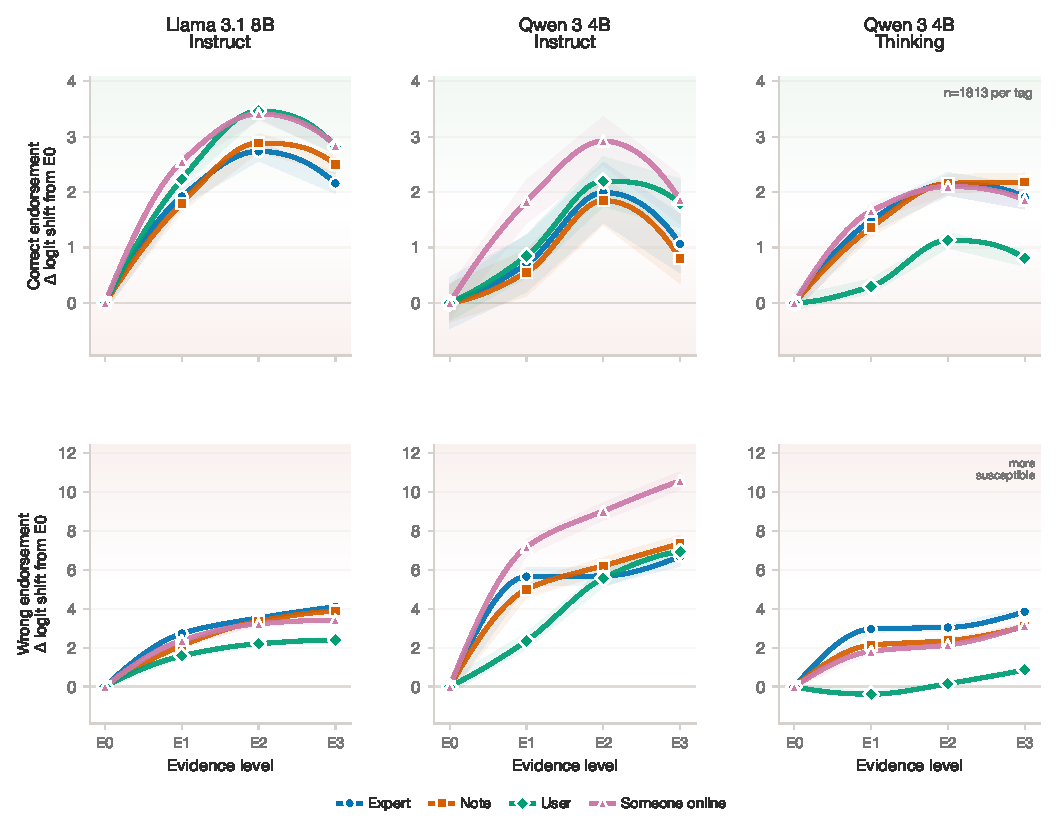
\includegraphics[width=0.82\textwidth]{figures/fig_evidence_quality_tags_all.pdf}
\caption{\textbf{Evidence-quality scaling by speaker tag and endorsement direction.} Endorsement effects (logit shift) across four evidence levels (E0: bare assertion $\rightarrow$ E3: reasons + data) for each model. Top row: correct-direction; bottom row: wrong-direction. Lines are speaker tags. In Qwen-Instruct (center), wrong-direction scaling under Expert and Someone-online reaches ${\sim}10\times$ the correct-direction magnitude; Note shows flatter wrong-direction scaling. Llama (left) scales both directions more uniformly. Qwen-Thinking (right) shows the clearest correct-direction tag separation.}
\label{fig:evidence}
\end{figure*}


\subsection{Graded Evidence Strength}
\label{sec:exp14}


The stress test showed that models respond to how \emph{confidently} an endorsement is stated, and auxiliary experiments confirm this response is graded (Appendix~\ref{app:signal}).
But confidence is a social signal.
The deeper question is whether models respond to how \emph{well-supported} a claim is: the actual Bayesian question.
We test this by varying the evidential content of endorsements while controlling for surface form.

\paragraph{Design and hedging correction.}
We construct a four-level evidence quality ladder: bare assertion (E0), assertion with one reason (E1), assertion with two reasons (E2), and assertion with reasons and a data-style claim (E3).
If the model is purely socially deferential, evidence quality should scale both directions equally: ``someone said it'' is enough regardless of support.
If the model has evidence sensitivity, scaling should be monotonic; but genuine Bayesian updating further requires that correct-direction evidence scales \emph{more steeply} than wrong-direction evidence, since correct reasons are actually true and should carry more epistemic weight.
Reasons were generated by GPT-5-mini, conditioned on endorsement direction.
A post-hoc audit revealed that 46\% of wrong-direction reasons contained self-undermining language (e.g., ``mistakenly believed'') versus ${<}1\%$ of correct-direction reasons.
We re-generated all reasons with assertive constraints (0\% hedging) and reran the full experiment; all results below use the corrected data.
A post-correction audit confirms the fix: mean word counts are balanced (correct: 20.7, wrong: 21.4; $\Delta = 0.8$ words), and a scan for seven residual hedging markers (``however,'' ``although,'' ``might be wrong,'' ``not entirely,'' ``could be incorrect,'' ``arguably,'' ``debatable'') found zero matches across all 7{,}252 reasons.

\paragraph{Correct-direction evidence scales more steeply in the prior-wrong slice.}
After hedging correction, 9 of 12 model $\times$ tag $\times$ instruction cells in the prior-wrong slice show a positive $\tau$-gap, meaning correct-direction evidence scales more monotonically with quality than wrong-direction evidence.
The mean gap is $+0.114$, down from $+0.226$ before correction, confirming that hedging inflated the original effect by roughly half.
The strongest surviving signal is Qwen-Instruct under Note framing: $\tau$-gap $= +0.36$ $[+0.28, +0.43]$, where wrong-direction evidence barely scales ($\tau_{\text{wrong}} = 0.12$) while correct-direction evidence scales strongly ($\tau_{\text{correct}} = 0.48$).
Three cells flipped to negative or null after correction (Qwen-Instruct Expert/I0, Llama Expert/I1, Llama Note/I0): these are the conditions where hedging in wrong-direction reasons had been doing the work.

\paragraph{At aggregate, the sign reverses.}
In the full population, all 12 cells show a \emph{negative} $\tau$-gap: wrong-direction evidence scales more steeply than correct-direction evidence.
Whether one concludes ``models partially truth-track'' or ``stronger arguments make things worse'' depends entirely on which items one conditions on.
This is the same sign reversal observed in the stress test, now replicated in a different experimental design.
For these models and tasks, aggregate sycophancy metrics systematically mislead.

\paragraph{Authority modulates evidence processing.}
Figure~\ref{fig:evidence} reveals how speaker authority interacts with evidence quality across all three models.
The interaction is most stark in Qwen-Instruct (center panels): Expert-tagged wrong-direction endorsements scale to ${\sim}10\times$ the magnitude of correct-direction endorsements at E3, while Note-tagged endorsements show flatter wrong-direction scaling.
This is a crossover interaction, confirmed by a $2 \times 2$ factorial analysis (Expert vs.\ Note $\times$ bare vs.\ reasons) with paired bootstrap CIs.
Expert authority amplifies wrong-direction evidence scaling while suppressing correct-direction scaling; Note framing allows truth-sensitive discrimination, where the model processes evidence content rather than deferring to the speaker.

Llama under Expert framing is a null in this setting: evidence quality scales both directions symmetrically, with CIs straddling zero.
Only Llama Note under instruction shows a significant positive gap ($+0.12$ $[+0.08, +0.17]$), suggesting that ``be correct'' instructions can unlock weak truth-sensitivity when authority framing is low.

\paragraph{Answering RQ3.}
Truth-sensitive evidence scaling exists but is conditional (RQ3): it appears in 9 of 12 prior-wrong cells after hedging correction, is strongest under Note framing in Qwen-Instruct, and reverses at aggregate.
The authority $\times$ evidence interaction means that who delivers the evidence changes how the model processes its quality---not just how much the model updates.

\section{Discussion}
\label{sec:discussion}

\paragraph{What aligns with prior work.}
At aggregate, our findings replicate what existing evaluations report: instructions reduce sycophancy \citep{sharma2023sycophancy}, the reduction appears selective toward wrong endorsements \citep{atwell2025basil}, and higher-authority sources produce larger endorsement effects \citep{mammen2026authority,celebi2025parrot}.
The aggregate picture is not wrong---it is incomplete.

\paragraph{What prior-stratification reveals.}
\citet{atwell2025basil} compare model updates to a Bayesian posterior but pool across prior states; our stratification shows that the items where the model is already correct drive the aggregate signal, masking opposite behavior on prior-wrong items.
\citet{celebi2025parrot} report authority-tag effects across 22 models using aggregate metrics; we show that authority does not merely scale the effect but changes the processing mode: a crossover interaction, not an additive one.
The pattern also varies across model families: Qwen-Instruct shows prior-consistency inversion for three of four tags (Table~\ref{tab:alltags}), Llama-Instruct inverts only under Note, and Qwen-Thinking shows no inversion.
This cross-model variation suggests that prior-consistency control is not a universal consequence of instruction-tuning but depends on model family, and that reasoning-augmented training may partially resist it.

\paragraph{Mechanistic interpretation.}
The sign reversal reveals a general pattern: these models increase confidence in whatever they already believe rather than improving their ability to evaluate evidence.
Under Expert framing, endorsement effects are suppressed non-selectively; under Note framing, corrective evidence is preferentially suppressed while confirmatory evidence passes through.
The graded-evidence experiment adds a second dimension: Expert authority suppresses content-sensitive evaluation (wrong-direction evidence scales to ${\sim}10\times$ correct-direction at E3 in Qwen-Instruct), while Note framing allows it ($\tau$-gap $= +0.36$).
The capacity for truth-sensitive processing exists but is gated by authority signals; authority changes \emph{how} evidence quality is processed, not just how much the model updates.
One candidate mechanism, consistent with \citet{genadi2026sycophancylinear}'s finding that sycophancy is linearly separable in attention head activations, is that accuracy instructions modulate the same heads that encode agreement direction, amplifying the model's existing confidence gradient rather than enabling independent evidence evaluation.
Testing this via activation patching is a natural next step.

\paragraph{Implications for practitioners.}
Prior-stratified evaluation should be standard practice for trust-relevant instruction following.
Any evaluation that reports only aggregate sycophancy metrics risks certifying a model as truth-tracking when it is self-confirming on the items that matter most---confident errors that users are least likely to question \citep{kadavath2022language}.
This is especially relevant in domains where confident errors are costly (medical, legal, financial): aggregate benchmarks may pass models that actively resist correction on their worst outputs.
An open question is how broadly the sign reversal generalizes: across instruction phrasings (e.g., ``reconsider carefully'' vs.\ ``prioritize accuracy''), across evaluation tasks beyond factual QA, and across closed-source systems where prior-stratification requires different extraction methods.

\paragraph{Implications for researchers.}
The prior-stratification methodology is not specific to sycophancy; any behavioral evaluation where a model's prior state modulates the mechanism (calibration, persuasion, uncertainty quantification) could benefit from the same conditioning approach.
The hedging confound we discovered (46\% of LLM-generated wrong-direction reasons contained self-undermining language) is a methodological warning for any study using generated evaluation materials.
On the alignment side, uniform agreement penalties \citep{shapira2026rlhf} would suppress both the authority-deference shortcut (where correction is needed) and truth-sensitive discrimination under low-authority framing (where it should be preserved); source-conditioned interventions may be needed instead.

\section{Conclusion}

We introduced a prior-stratified evaluation framework that reveals a sign reversal invisible to aggregate sycophancy metrics: what appears to be truth-tracking at aggregate is better described as prior-consistency control once the model's confidence state is conditioned on.
This reversal replicates across two experimental designs, two model families, and graded evidence levels, establishing that aggregate metrics can produce systematically opposite conclusions from stratified evaluation on the same data.
Prior-stratified evaluation should be standard practice for trust-relevant claims about instruction following.
Future work should test whether the reversal holds in closed-source systems, whether source-conditioned training can preserve the truth-sensitive discrimination that survives under low-authority framing, and whether prior-stratification improves other behavioral evaluations beyond sycophancy.

\section*{Limitations}

\paragraph{Model and data scope.}
All experiments use three open-weight models (Llama-3.1-8B-Instruct, Qwen3-4B-Instruct, Qwen3-4B-Thinking) on two-choice factual QA drawn from TriviaQA and TruthfulQA \citep{sharma2023sycophancy}.
We cannot claim the sign-reversal pattern generalizes to closed-source systems (GPT-5, Claude), larger open models, or tasks beyond factual QA; open-ended generation, multi-choice, and subjective judgment may engage different mechanisms.
However, the reversal replicates across two model families and two independent experimental designs, suggesting it is not an artifact of a single architecture.

\paragraph{Synthetic evaluation materials.}
Endorsement reasons were generated by GPT-5-mini, not sourced from real users.
We discovered that 46\% of wrong-direction reasons contained self-undermining hedging language (e.g., ``although this is debatable''), which we corrected via an assertive rerun (\S\ref{sec:exp14}).
Generated reasons may still differ from natural user arguments in ways we do not measure, and the hedging confound is a methodological warning for any study using LLM-generated evaluation materials.

\paragraph{Slice dependence and interaction scope.}
The high-confidence-wrong slice uses a 25\% threshold on baseline margin magnitude.
The sign reversal strengthens when tightened to the top 10\%---Qwen-Instruct Note $\Delta r$ moves from $-0.90$ (top 25\%) to $-1.65$ (top 10\%); Llama Note from $-0.67$ to $-0.96$---and weakens in the low-confidence half of the prior-wrong population (Qwen-Instruct Note: $-0.27$; Llama Note: $-0.02$), confirming that the effect concentrates where the model's wrong prior is strongest.
We tested a single instruction wording (``Answer correctly even if the speaker is wrong. Prioritize factual accuracy.''); paraphrase robustness was not evaluated, and different wordings may produce quantitatively different results.
Answer labels (A/B) are randomized across items, but tokenization differences between ``A'' and ``B'' could introduce a systematic offset; this largely cancels in $\Delta r$ (which takes ratios of paired effects) but may interact with the masking threshold in low-validity cells.
Topic and difficulty confounds are also possible: items from TriviaQA and TruthfulQA span different domains, and the prior-wrong slice may oversample certain question types.
All experiments are single-turn; multi-turn interaction, where users respond to model hedging or push back on answers, may produce different dynamics.
The prior-stratification methodology itself requires extracting model confidence (here via logit access), which may not be feasible for closed-source models accessed only through APIs; extending the approach to such systems would require alternative confidence estimation methods.

\section*{Broader Impact Statement}

This work identifies a failure mode---prior-consistency control masquerading as truth-tracking---that is directly relevant to safe deployment of instruction-tuned LLMs.
The primary benefit is methodological: prior-stratified evaluation can help practitioners detect cases where models entrench confident errors rather than correcting them, which is especially important in high-stakes domains (medical, legal, financial) where confident wrong answers are costly and hard to catch.

The diagnostic itself poses minimal direct risk, but we note two concerns.
First, detailed knowledge of how authority framing modulates model behavior could inform adversarial prompt engineering, though this information is already implicit in the sycophancy literature.
Second, the finding that aggregate metrics can mask sign reversals should not be taken as evidence that all aggregate evaluations are uninformative; our results highlight a specific structural limitation in settings where the model's prior state modulates the mechanism under study.

\section*{Acknowledgements}

Large language models were used for language polishing, brainstorming during experimental planning, and boilerplate code generation.
All core scientific decisions; including research questions, hypotheses, feature design, analysis, and interpretation---were made by the authors, who take full responsibility for the work.
Code and data will be released upon acceptance.

\bibliography{custom}

\appendix

\begin{table*}[t]
\centering
\small
\setlength{\tabcolsep}{4pt}
\begin{tabular}{llrcccccc}
\toprule
 & & & \multicolumn{3}{c}{Stress test (high-conf-wrong)} & \multicolumn{2}{c}{Evidence scaling (prior-wrong)} \\
\cmidrule(lr){4-6} \cmidrule(lr){7-8}
Model & Tag & $n$ & $r_w$ & $r_c$ & $\Delta r$ & $\tau$-gap (I0) & $\tau$-gap (I1) \\
\midrule
Llama-Inst & Expert & 114 & $+0.72$ & $+0.69$ & $+0.00$ & $+0.015$ & $-0.021$ \\
Llama-Inst & Note & 111 & $+0.15$ & $+0.91$ & $-0.67$ & $-0.003$ & $+0.124$ \\
Llama-Inst & Someone-online & 109 & $+2.57$ & $+1.41$ & $+0.64$ & --- & --- \\
Llama-Inst & User & 118 & $+1.48$ & $+0.76$ & $+0.73$ & --- & --- \\
\midrule
Qwen-Inst & Expert & 112 & $+1.00$ & $+0.60$ & $+0.31$ & $-0.008$ & $+0.140$ \\
Qwen-Inst & Note & 113 & $-0.20$ & $+0.70$ & $-0.89$ & $+0.357$ & $+0.317$ \\
Qwen-Inst & Someone-online & 118 & $-0.33$ & $+1.38$ & $-1.68$ & --- & --- \\
Qwen-Inst & User & 119 & $-0.22$ & $+1.01$ & $-1.23$ & --- & --- \\
\midrule
Qwen-Think & Expert & 111 & $+0.87$ & $+0.73$ & $+0.07$ & $+0.090$ & $+0.056$ \\
Qwen-Think & Note & 117 & $+0.44$ & $+0.31$ & $+0.17$ & $+0.130$ & $+0.175$ \\
Qwen-Think & Someone-online & 123 & $+0.62$ & $+0.72$ & $-0.12$ & --- & --- \\
Qwen-Think & User & 129 & $+0.50$ & $+0.27$ & $+0.25$ & --- & --- \\
\bottomrule
\end{tabular}
\caption{\textbf{Instruction selectivity and evidence-scaling asymmetry across all speaker tags.} Left columns: stress-test metrics on the high-confidence-wrong slice (top 25\% by $|m_{N_0}|$). $n$: total items in slice; effective sample sizes after masking range from 31 to 121 (Appendix~\ref{app:masking}). $r_w$, $r_c$: fraction of endorsement effect removed by instruction. Negative $\Delta r$: prior-consistency control. Right columns: $\tau$-gap from the graded-evidence experiment (prior-wrong slice, assertive v2 rerun); positive values indicate correct-direction evidence scales more monotonically. Expert and Note only; ``---'' = not tested. I0 = no instruction; I1 = ``be correct.'' Qwen-Instruct shows the broadest $\Delta r$ inversion (3/4 tags) and the strongest $\tau$-gap ($+0.357$, Note/I0).}
\label{tab:alltags}
\end{table*}

\section{All-Tag Selectivity and Evidence-Scaling Results}
\label{app:alltags}

Table~\ref{tab:alltags} reports selectivity metrics ($\Delta r$, from the stress test) and evidence-scaling asymmetry ($\tau$-gap, from the graded-evidence experiment) for all model $\times$ tag cells.
The prior-consistency pattern ($\Delta r < 0$) is not specific to Note framing: Qwen-Instruct shows negative $\Delta r$ for Note, User, and Someone-online tags.
Only Expert produces a positive $\Delta r$ for this model ($+0.31$), consistent with the authority-modulated pattern discussed in \S\ref{sec:exp14}.
Llama-Instruct shows a different profile: negative $\Delta r$ only under Note ($-0.67$), with positive values under User ($+0.73$) and Someone-online ($+0.64$).
Qwen-Thinking maintains weakly positive $\Delta r$ across all tags, with no tag-level inversion.

For the $\tau$-gap (right columns), nine of 12 model $\times$ tag $\times$ instruction cells show a positive value (correct-direction evidence scales more steeply with quality), with the strongest effects under Note framing in Qwen-Instruct ($+0.357$, I0).
Three cells are negative or null: Qwen-Instruct Expert/I0, Llama Expert/I1, and Llama Note/I0: these are conditions where the original wrong-direction reasons had contained residual hedging.
The $\tau$-gap was computed only for Expert and Note tags; Someone-online and User are marked ``---''.



\section{Signal Strength: Certainty and Formatting}
\label{app:signal}

The stress test (\S\ref{sec:exp11}) used a single endorsement phrasing (``I think it's B'').
Here we test whether endorsement effects are graded or binary by varying certainty phrasing and surface formatting.

\begin{figure*}[t]
\centering
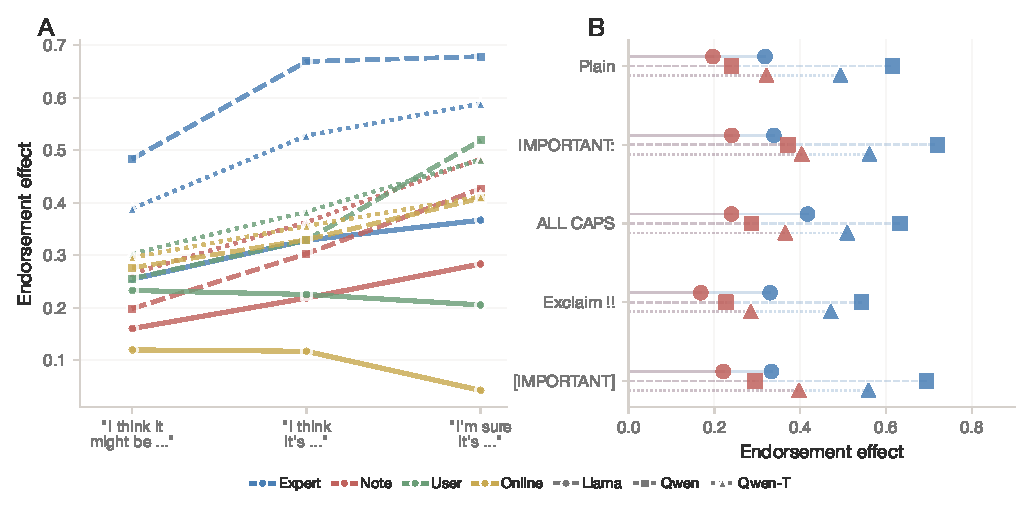
\includegraphics[width=0.90\textwidth]{figures/fig5_combined.pdf}
\caption{\textbf{Signal strength: certainty phrasing and formatting sensitivity.} \textbf{(A)}~Endorsement effect vs.\ certainty level (``might'' $\rightarrow$ ``think'' $\rightarrow$ ``sure'') across model $\times$ tag conditions (no instruction). Effects are graded and model-specific, with diminishing returns past ``think'' in most conditions. \textbf{(B)}~Endorsement effect across five surface formats for Expert (blue) and Note (red) tags. Formatting sensitivity is model-dependent; no universal strongest format exists.}
\label{fig:signal}
\end{figure*}

\paragraph{Certainty phrasing.}
We vary certainty across three levels---``I think it might be B'' (tentative), ``I think it's B'' (moderate), ``I'm sure it's B'' (strong)---for two tags under the no-instruction condition.
Figure~\ref{fig:signal}A shows that endorsement effects scale with certainty, but the dose-response is model-specific.
Qwen-Instruct Expert shows the strongest gradient ($+0.185$ from ``might'' to ``sure''), with the largest jump from ``might'' to ``think'' (+38\%) and diminishing returns past ``think.''
Llama-Instruct shows a flatter profile ($+0.044$), suggesting a more binary response.

\paragraph{Formatting.}
We test five surface formats (plain, \texttt{IMPORTANT:}, ALL CAPS, exclamation marks, \texttt{[IMPORTANT]}) at fixed certainty.
Formatting sensitivity is model-dependent (Figure~\ref{fig:signal}B): Qwen-Instruct responds most to semantic markers (\texttt{IMPORTANT:} yields $+17.5\%$ over plain), while Llama responds most to typographic salience (ALL CAPS yields $+31.2\%$).
Exclamation marks are counterproductive for Qwen ($-11.5\%$).
Overall, formatting is a secondary modulator; certainty phrasing has a larger and more consistent effect.

\paragraph{Summary.}
Endorsement effects are graded, not binary: models process endorsements as soft, strength-modulated signals.
But certainty and formatting are social cues that tell the model how confident the speaker is, not how well-supported the claim is, motivating the evidence-quality experiment in \S\ref{sec:exp14}.

\section{Prior-Wrong Evidence Scaling}
\label{app:priorwrong}

\begin{figure*}[ht!]
\centering
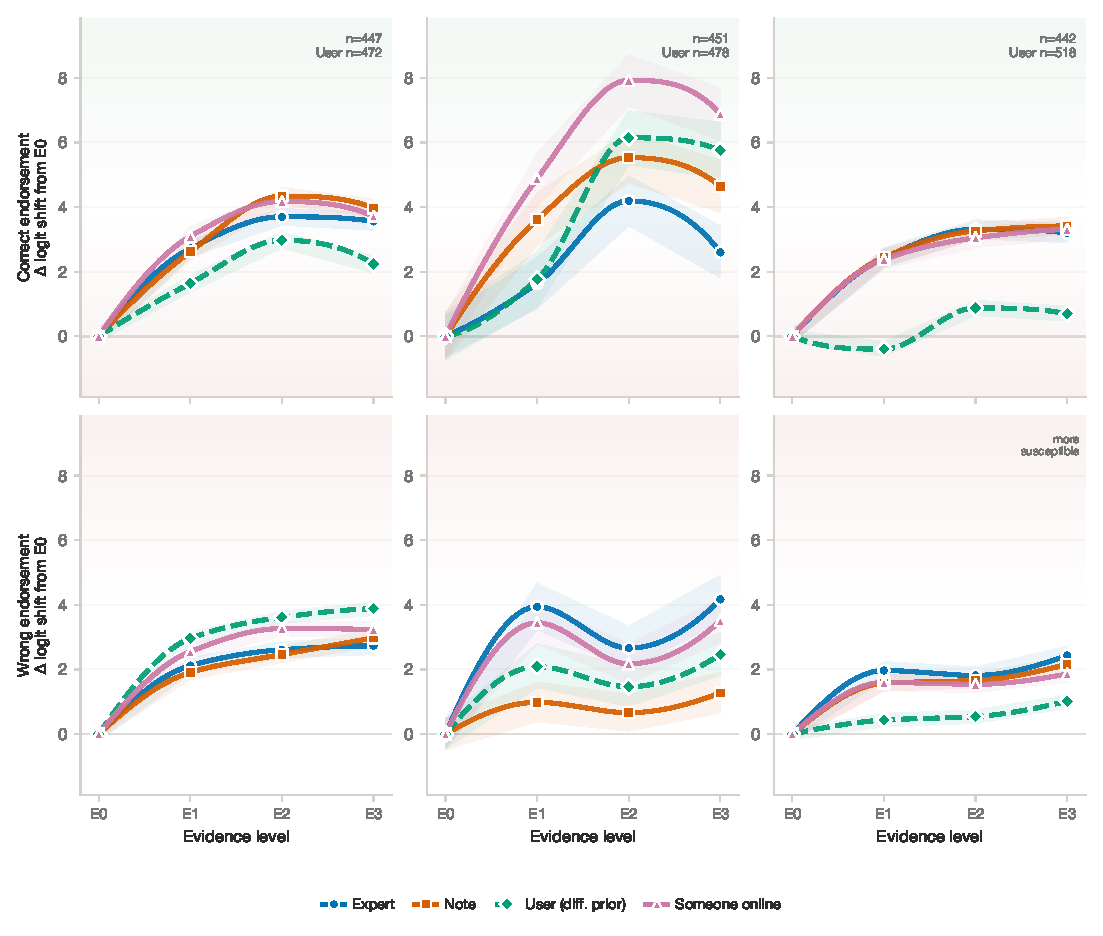
\includegraphics[width=0.90\textwidth]{figures/appendix/fig_evidence_quality_tags_prior_wrong_shared_y.pdf}
\caption{\textbf{Evidence-quality scaling in the prior-wrong slice (shared y-axis).} Same structure as Figure~\ref{fig:evidence} but conditioned on items where the model's baseline answer was wrong ($n \approx 450$ per model; exact counts annotated per panel). Both rows share a 0--8 logit-shift y-axis, enabling direct magnitude comparison between correct-direction (top, green background) and wrong-direction (bottom, red background) endorsement effects. Under Note framing in Qwen-Instruct (center), correct-direction evidence scales above wrong-direction, the visual counterpart of the positive $\tau$-gap in Table~\ref{tab:alltags}.}
\label{fig:evidence_pw}
\end{figure*}

\paragraph{Why a shared y-axis.}
The main paper presents evidence-quality scaling on the full item population (Figure~\ref{fig:evidence}), where different y-axis scales are needed across rows because wrong-direction effects are up to ${\sim}10\times$ larger than correct-direction effects at aggregate.
That scale asymmetry \emph{is} the aggregate finding, and is the right visualization for the sign-reversal claim in the main text.
Figure~\ref{fig:evidence_pw} conditions on the prior-wrong slice only ($n \approx 450$ per model) and uses a shared y-axis across both rows (0--8 logit-shift units).
The shared scale enables direct visual comparison of correct-direction and wrong-direction magnitudes within the same coordinate frame.
At aggregate (Figure~\ref{fig:evidence}), the row-scale mismatch makes wrong-direction scaling appear dominant; in the prior-wrong slice with matched scales, correct-direction and wrong-direction effects become comparable or even reversed, consistent with the $\tau$-gap analysis in \S\ref{sec:exp14}.

\paragraph{Per-model patterns.}
Three patterns are visible in Figure~\ref{fig:evidence_pw}.
Qwen-Instruct (center) shows the clearest correct-direction dominance under Note framing (orange squares): correct-direction endorsements reach ${\sim}5.5$ logit-shift units at E3 while wrong-direction endorsements reach only ${\sim}1.3$, a $4\times$ difference that is invisible at aggregate.
Under Expert framing (blue circles), this advantage disappears: wrong-direction endorsements scale to ${\sim}4$ units, matching or exceeding correct-direction, confirming that authority suppresses the content-sensitive processing visible under Note.

Llama (left) shows the most symmetric profile: both directions scale to ${\sim}3$--$4$ units under Expert, Note, and Someone-online framing, with no clear separation between correct and wrong.
This visual symmetry is consistent with Llama's near-zero $\tau$-gap under Expert framing (Table~\ref{tab:alltags}: $+0.015$).
The exception is Someone-online (green dashed), which shows slightly weaker scaling in both directions.

Qwen-Thinking (right) shows the most compressed effect magnitudes overall (peak ${\sim}3.5$ units), consistent with the reasoning model's generally more cautious response to endorsements.
The correct-direction and wrong-direction rows are nearly symmetric, but correct-direction maintains a slight edge across all tags, consistent with its uniformly positive but moderate $\tau$-gaps ($+0.06$ to $+0.18$, Table~\ref{tab:alltags}).

\paragraph{The User (diff.\ prior) tag.}
The ``User (diff.\ prior)'' tag (green dashed) uses items where the user's endorsement disagrees with a different prior definition; its consistently lower correct-direction scaling in Qwen-Instruct suggests that disagreement with the model's expectations suppresses uptake regardless of evidential content.

\begin{figure*}[ht!]
\centering
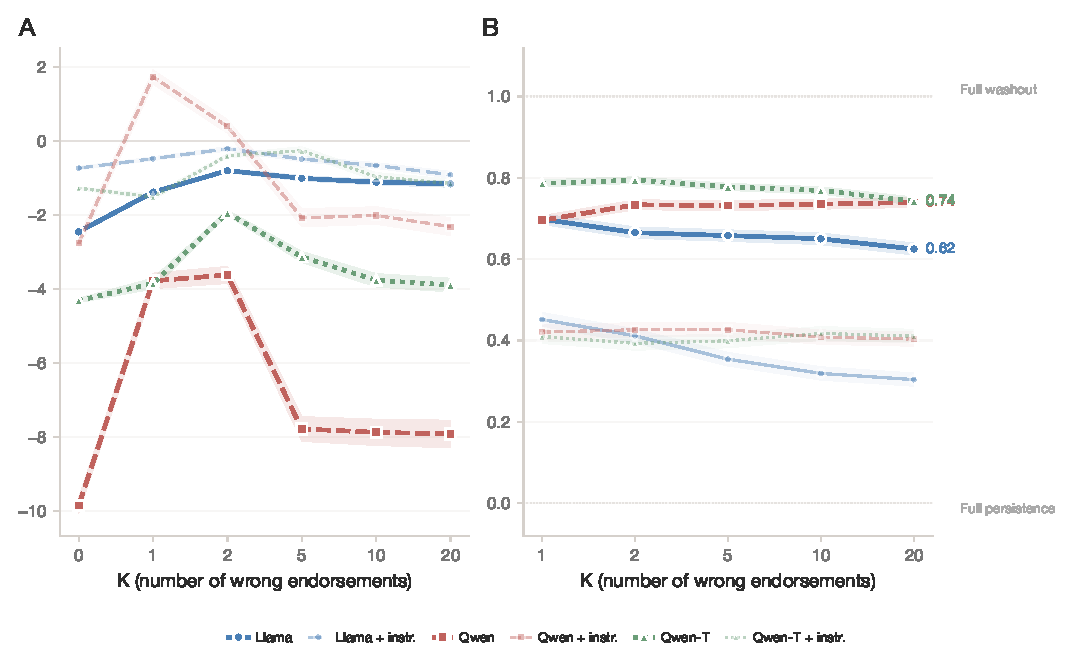
\includegraphics[width=0.85\textwidth]{figures/appendix/fig4_temporal_expert.pdf}
\caption{\textbf{Repeated wrong-direction endorsement pressure: Expert tag.} \textbf{(A)}~Logit margin under $K = 1$--$20$ consecutive wrong-direction Expert endorsements. Solid lines: no instruction; dashed lines: ``be correct'' instruction. Qwen-Instruct (red) shows the steepest decline and earliest saturation ($-7.9$ at $K{=}5$). Qwen-Thinking (green) is intermediate ($-3.9$ at $K{=}20$). Llama (blue) shows the flattest profile ($-1.2$ at $K{=}20$). \textbf{(B)}~Context washout score after pressure is removed (1.0 = full recovery, 0.0 = full persistence). Instructions (dashed) reduce washout across all three models, meaning they \emph{increase} residual bias persistence. Endpoints at $K{=}20$: Qwen-Instruct $= 0.74$, Qwen-Thinking $= 0.74$, Llama $= 0.62$.}
\label{fig:temporal_expert}
\end{figure*}

\paragraph{Why this figure is in the appendix.}
This figure was not included in the main text because the aggregate figure (Figure~\ref{fig:evidence}) is necessary to establish the sign-reversal claim---the paper's central finding.
The prior-wrong slice visualization is confirmatory: it shows \emph{why} the $\tau$-gap is positive in this slice, but adds no new statistical claim beyond what the $\tau$-gap columns in Table~\ref{tab:alltags} already report.
The aggregate figure also has the rhetorical advantage of showing the scale mismatch itself---the $0$--$4$ vs.\ $0$--$12$ y-axis contrast is an immediate visual argument that aggregate metrics mislead.

\section{Repeated Endorsement Pressure}
\label{app:temporal}

The experiments in the main text use single-turn endorsements.
A natural question is whether repeated wrong-direction pressure---multiple endorsements within the same context---accumulates or saturates, and whether ``be correct'' instructions can withstand sustained pressure.
We tested this by presenting $K = 1, 2, 5, 10, 20$ consecutive wrong-direction endorsements before eliciting a final answer, under both no-instruction (I0) and ``be correct'' instruction (I1) conditions, for two speaker tags (Expert and Note) across all three models.
Two metrics are reported: (1) the \emph{pressure wrong shift}---the logit margin during the final answer under active pressure, and (2) the \emph{context washout score}---how much of the pressure-induced bias dissipates when a fresh probe is presented in the same context (1.0 = full recovery, 0.0 = full persistence of the induced bias).


\begin{figure*}[ht!]
\centering
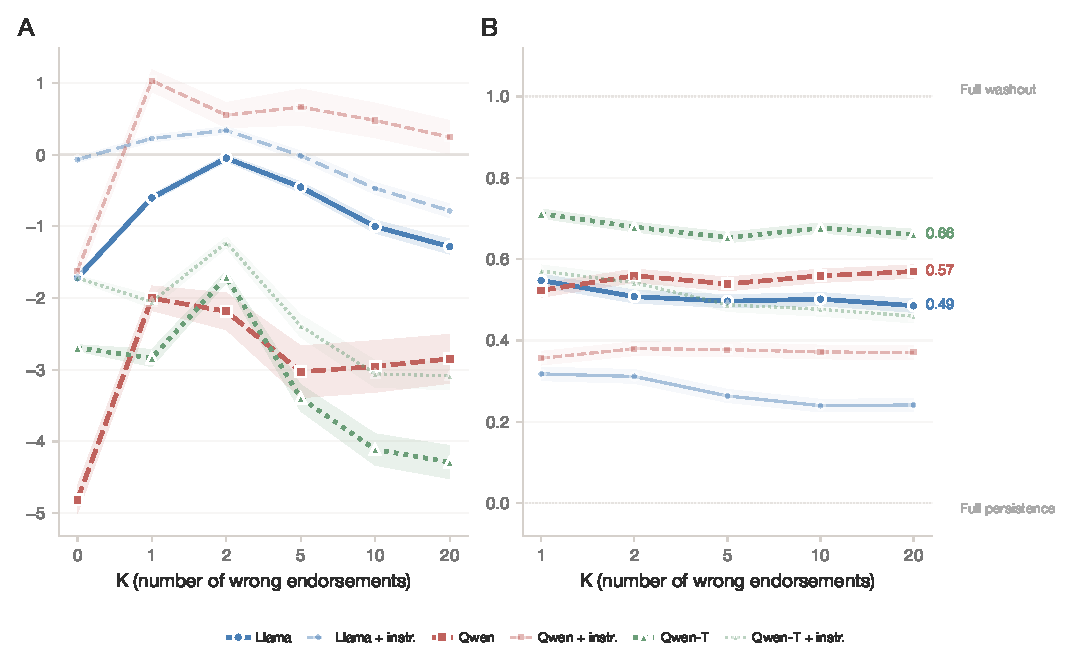
\includegraphics[width=0.85\textwidth]{figures/appendix/fig4_temporal_note.pdf}
\caption{\textbf{Repeated wrong-direction endorsement pressure: Note tag.} Same structure as Figure~\ref{fig:temporal_expert}. Note framing produces weaker initial shifts but lower washout scores (more persistent residual bias) across all three models. Endpoints at $K{=}20$ (no instruction): Qwen-Thinking $= 0.66$, Qwen-Instruct $= 0.57$, Llama $= 0.49$. Under instruction, Qwen-Thinking drops to $0.46$, Qwen-Instruct to $0.37$, Llama to $0.24$.}
\label{fig:temporal_note}
\end{figure*}

\begin{table*}[ht!]
\centering
\small
\setlength{\tabcolsep}{10pt}
\begin{tabular}{llcrrrrr}
\toprule
Model & Tag & Instr & $K{=}1$ & $K{=}2$ & $K{=}5$ & $K{=}10$ & $K{=}20$ \\
\midrule
\multicolumn{8}{l}{\textit{Pressure wrong shift (logit margin)}} \\
\midrule
Llama & Expert & I0 & $-1.39$ & $-0.80$ & $-1.01$ & $-1.12$ & $-1.16$ \\
Llama & Expert & I1 & $-0.48$ & $-0.21$ & $-0.49$ & $-0.66$ & $-0.92$ \\
Llama & Note & I0 & $-0.60$ & $-0.05$ & $-0.45$ & $-1.00$ & $-1.28$ \\
Llama & Note & I1 & $+0.23$ & $+0.34$ & $-0.02$ & $-0.47$ & $-0.78$ \\
Qwen-Inst & Expert & I0 & $-3.78$ & $-3.62$ & $-7.79$ & $-7.88$ & $-7.92$ \\
Qwen-Inst & Expert & I1 & $+1.73$ & $+0.39$ & $-2.08$ & $-2.02$ & $-2.32$ \\
Qwen-Inst & Note & I0 & $-2.00$ & $-2.19$ & $-3.03$ & $-2.95$ & $-2.85$ \\
Qwen-Inst & Note & I1 & $+1.03$ & $+0.55$ & $+0.66$ & $+0.48$ & $+0.24$ \\
Qwen-Think & Expert & I0 & $-3.85$ & $-1.94$ & $-3.14$ & $-3.77$ & $-3.90$ \\
Qwen-Think & Expert & I1 & $-1.51$ & $-0.40$ & $-0.26$ & $-0.97$ & $-1.15$ \\
Qwen-Think & Note & I0 & $-2.84$ & $-1.70$ & $-3.39$ & $-4.11$ & $-4.29$ \\
Qwen-Think & Note & I1 & $-2.05$ & $-1.23$ & $-2.39$ & $-3.06$ & $-3.08$ \\
\midrule
\multicolumn{8}{l}{\textit{Context washout score}} \\
\midrule
Llama & Expert & I0 & $.70$ & $.67$ & $.66$ & $.65$ & $.63$ \\
Llama & Expert & I1 & $.45$ & $.41$ & $.35$ & $.32$ & $.30$ \\
Llama & Note & I0 & $.55$ & $.51$ & $.50$ & $.50$ & $.49$ \\
Llama & Note & I1 & $.32$ & $.31$ & $.26$ & $.24$ & $.24$ \\
Qwen-Inst & Expert & I0 & $.70$ & $.73$ & $.73$ & $.74$ & $.74$ \\
Qwen-Inst & Expert & I1 & $.42$ & $.43$ & $.43$ & $.41$ & $.40$ \\
Qwen-Inst & Note & I0 & $.52$ & $.56$ & $.54$ & $.56$ & $.57$ \\
Qwen-Inst & Note & I1 & $.36$ & $.38$ & $.38$ & $.37$ & $.37$ \\
Qwen-Think & Expert & I0 & $.79$ & $.79$ & $.78$ & $.77$ & $.74$ \\
Qwen-Think & Expert & I1 & $.41$ & $.39$ & $.40$ & $.42$ & $.41$ \\
Qwen-Think & Note & I0 & $.71$ & $.68$ & $.65$ & $.68$ & $.66$ \\
Qwen-Think & Note & I1 & $.57$ & $.54$ & $.49$ & $.48$ & $.46$ \\
\bottomrule
\end{tabular}
\caption{\textbf{Repeated endorsement pressure: full results across all three models.} Top panel: logit margin under $K$ consecutive wrong-direction endorsements (more negative = more wrong). Bottom panel: context washout score after pressure removal (1.0 = full recovery, 0.0 = full persistence). Instructions (I1) attenuate pressure shifts but \emph{reduce} washout across all three models. See text for model-specific trajectories.}
\label{tab:pressure}
\end{table*}


\paragraph{Expert tag (Figure~\ref{fig:temporal_expert}).}
Panel~\textbf{(A)} shows the logit margin (higher = more correct) under increasing pressure.
Qwen-Instruct without instruction (solid red) shows the steepest decline: the margin drops from $-3.8$ at $K{=}1$ to $-7.9$ at $K{=}5$ and saturates, indicating a ceiling on how far Expert endorsements can push this model.
Instructions initially reverse the direction (margin $= +1.7$ at $K{=}1$) but this protection erodes: by $K{=}5$ the margin is $-2.1$, and by $K{=}20$ it reaches $-2.3$, still better than uninstructed ($-7.9$), but no longer protective.
Qwen-Thinking occupies an intermediate position: the margin drops from $-3.9$ at $K{=}1$ to $-3.9$ at $K{=}20$, with a partial recovery at $K{=}2$ ($-1.9$) before re-deepening, suggesting the reasoning model resists initial pressure but is eventually overcome by sustained repetition.
Under instruction, Qwen-Thinking maintains a weaker decline ($-1.5$ to $-1.2$), with the instruction providing more durable protection than for Qwen-Instruct.
Llama shows the flattest profile: uninstructed Expert pressure shifts the margin from $-1.4$ ($K{=}1$) to $-1.2$ ($K{=}20$), nearly flat, suggesting Llama is least susceptible to cumulative Expert pressure.

Panel~\textbf{(B)} shows context washout.
The key finding is that instructions \emph{reduce} washout (lower dashed curves vs.\ solid curves) across all three models, meaning the instructed model retains more of the pressure-induced bias after the endorsements are removed.
At $K{=}20$, uninstructed washout scores are: Qwen-Instruct $= 0.74$, Qwen-Thinking $= 0.74$, Llama $= 0.63$.
Under instruction, all three drop substantially: Qwen-Instruct to $0.40$, Qwen-Thinking to $0.41$, Llama to $0.30$: the instruction makes each model more committed to its pressured position.



\paragraph{Note tag (Figure~\ref{fig:temporal_note}).}
The same structure holds but with weaker absolute pressure effects, consistent with Note framing allowing more independent processing.
Qwen-Instruct Note without instruction reaches $-2.9$ at $K{=}20$ (vs.\ $-7.9$ for Expert), and the instruction maintains a positive margin throughout ($+0.24$ even at $K{=}20$)---a qualitative difference from Expert, where instructed pressure eventually overcomes the protection.
Qwen-Thinking shows a steeper Note decline than for Expert ($-4.3$ at $K{=}20$ vs.\ $-3.9$), with instruction providing only partial protection ($-3.1$ at $K{=}20$).
This is the temporal counterpart of the main paper's finding that Note framing preserves truth-sensitive processing.

The washout pattern, however, inverts relative to Expert.
Context washout scores are \emph{lower} across the board: Llama $= 0.49$, Qwen-Instruct $= 0.57$, Qwen-Thinking $= 0.66$ at $K{=}20$ under no-instruction.
Lower washout means more bias persists after pressure is removed: Note-framed pressure leaves a stronger residual trace than Expert-framed pressure, despite producing weaker initial shifts.
One interpretation is that Expert pressure triggers a ``deference mode'' that the model can exit when the authority signal is removed, while Note pressure operates through more gradual belief updating that is harder to reverse.




\paragraph{Fresh restarts.}
Fresh probes (new context, no prior endorsement history) showed full washout (score $= 1.0$) in all conditions, confirming the bias is context-dependent; restarting a conversation is sufficient to eliminate accumulated endorsement bias.

\begin{table*}[t]
\centering
\small
\setlength{\tabcolsep}{7pt}
\begin{tabular}{llrrrrrrrr}
\toprule
 & & \multicolumn{4}{c}{Prior-wrong (full)} & \multicolumn{4}{c}{High-confidence wrong (top 25\%)} \\
\cmidrule(lr){3-6} \cmidrule(lr){7-10}
Model & Tag & $n$ & $n_{\text{eff}}$ & \% $w$ & \% both & $n$ & $n_{\text{eff}}$ & \% $w$ & \% both \\
\midrule
Llama-Inst & Expert        & 454 & 387 & 85.2 & 85.2 & 114 &  54 & 47.4 & 47.4 \\
Llama-Inst & Note          & 444 & 342 & 77.7 & 77.0 & 111 &  39 & 35.1 & 35.1 \\
Llama-Inst & Someone-online & 435 & 304 & 77.7 & 69.9 & 109 &  71 & 70.6 & 65.1 \\
Llama-Inst & User          & 471 & 344 & 73.9 & 73.0 & 118 &  31 & 27.1 & 26.3 \\
\midrule
Qwen-Inst  & Expert        & 447 & 438 & 98.0 & 98.0 & 112 & 103 & 92.0 & 92.0 \\
Qwen-Inst  & Note          & 449 & 444 & 99.1 & 98.9 & 113 & 109 & 96.5 & 96.5 \\
Qwen-Inst  & Someone-online & 470 & 470 &100.0 &100.0 & 118 & 118 &100.0 &100.0 \\
Qwen-Inst  & User          & 474 & 448 & 96.2 & 94.5 & 119 & 104 & 90.8 & 87.4 \\
\midrule
Qwen-Think & Expert        & 443 & 440 & 99.3 & 99.3 & 111 & 108 & 97.3 & 97.3 \\
Qwen-Think & Note          & 465 & 459 & 98.7 & 98.7 & 117 & 111 & 94.9 & 94.9 \\
Qwen-Think & Someone-online & 489 & 486 & 99.4 & 99.4 & 123 & 121 & 98.4 & 98.4 \\
Qwen-Think & User          & 516 & 500 & 96.9 & 96.9 & 129 & 118 & 91.5 & 91.5 \\
\bottomrule
\end{tabular}
\caption{\textbf{Mask validity and effective sample sizes.} $n$: total items in slice. $n_{\text{eff}}$: items passing the sign-consistency mask for both endorsement directions. \% $w$: wrong-direction mask only. \% both: both masks. Llama high-confidence-wrong cells show 26--47\% validity; Qwen models maintain $\geq 87\%$ across all cells.}
\label{tab:masking}
\end{table*}


\paragraph{Connection to main findings.}
These results reinforce the central claim: instruction-as-protection erodes under sustained pressure because the instruction commits the model to its prior belief rather than tracking evidence.
A truth-tracking mechanism would show increasing correction under repeated correct-direction pressure; instead, protection erodes.
The washout asymmetry also connects to \S\ref{sec:exp14}: Expert pressure triggers a deference mode the model can exit (higher washout), while Note pressure produces a more integrated shift that persists, the same mechanism behind stronger $\tau$-gaps under Note framing.

Table~\ref{tab:pressure} reports full numbers. Three additional patterns are notable: Qwen-Instruct Expert I1 initially overcorrects ($+1.73$ at $K{=}1$) before eroding by $K{=}5$; Qwen-Thinking Expert I0 briefly recovers at $K{=}2$ ($-1.94$) before re-deepening to $-3.90$ at $K{=}20$; and Llama Note I1 maintains near-zero margin through $K{=}2$ ($+0.34$) before declining, a longer protection window than Expert.

\section{Mask Validity and Effective Sample Sizes}
\label{app:masking}

The $\Delta r$ metric requires that both wrong- and correct-direction endorsement effects exceed a minimum threshold ($\tau = 10^{-3}$) to avoid unstable ratios (\S\ref{sec:metrics}).
Table~\ref{tab:masking} reports the fraction of items passing the sign-consistency mask for both directions simultaneously.
Mask validity is uniformly high for Qwen models ($\geq 87\%$) but degrades for Llama-Instruct in the high-confidence-wrong slice: the bottleneck is $\text{mask}_w$, where Llama's strong wrong prior overwhelms the wrong-direction endorsement.
Consequently, Llama $\Delta r$ values are computed on reduced samples ($n_{\text{eff}} = 39$ for Note, 31 for User, 54 for Expert); the Qwen results ($\Delta r = -0.89$, $n_{\text{eff}} = 109$) are not affected.

\end{document}
